\chapter{Specifikacija programske potpore}
		
	\section{Funkcionalni zahtjevi}
			
			\noindent \textbf{Dionici:}
			
			\begin{packed_enum}
				
				\item Korisnici
				\item Admini sustava				
				\item Razvojni tim
				
			\end{packed_enum}
			
			\noindent \textbf{Aktori i njihovi funkcionalni zahtjevi:}
			
			
			\begin{packed_enum}
				\item  \underbar{Zaposlenik (inicijator) može:}
				
				\begin{packed_enum}
					
					\item učitavati slike
					\item skenirati dokumente
					\item pregledati povijest skeniranih dokumenata
					\item slati dokumente revizoru
					
				\end{packed_enum}
			
				\item  \underbar{Revizor (sudionik) može:}
				
				\begin{packed_enum}
					
					\item skenirati dokument
					\item provjeriti jeli dokumenat ispravan i poslati ga računovođi
					
				\end{packed_enum}
			
				\item  \underbar{Računovođa (sudionik) može:}
				
				\begin{packed_enum}
					
					\item dodjeljivati jedinstveni broj arhivu
					\item arhivirati dokument
					\item slati obavijest direktoru da se potpiše dokument
					
				\end{packed_enum}
			
				\item  \underbar{Direktor (sudionik) može:}
				
				\begin{packed_enum}
					
					\item potpisati dokumente i poslati obavijest da je dokument potpisan
					\item pregledati povijest svih dokumenata
					\item pregledati statistiku svih zaposlenika
					
				\end{packed_enum}
				
				\item  \underbar{Baza podataka (sudionik) može:}
				
				\begin{packed_enum}
					
					\item dodati nove dokumente i arhive u bazu
					\item vraćati povijest svih dokumenata
					\item vraćati statistiku svih zaposlenika
					
				\end{packed_enum}	
			
			\end{packed_enum}
			
			
			\eject 
			
			
				
			\subsection{Obrasci uporabe}
				
				
				\subsubsection{Opis obrazaca uporabe}
				
						\noindent \underbar{\textbf{UC1 - Prijava korisnika  }}
					\begin{packed_item}
						
						\item \textbf{Glavni sudionik:} Zaposlenik
						\item  \textbf{Cilj:} Omogućiti prijavu postojećim korisnicima ili odabrati registraciju novih
						\item  \textbf{Sudionici:} Baza podataka
						\item  \textbf{Preduvjet:} U bazi podataka mora postojati račun korisnika, odnosno direktor mora odobriti registraciju
						\item  \textbf{Opis osnovnog tijeka:}
						
						\item[] \begin{packed_enum}
							
							\item Korisnik unosi svoje korisničke detalje i nakon provjere ulazi u home page
							\item Nepostojeći korisnici imaju opciju preusmjeravanja na registraciju
							
						\end{packed_enum}
						\item  \textbf{Opis mogućih odstupanja:}
						
						\item[] \begin{packed_item}
							
							\item[2.a] Korisnik je unio korisničke detalje koji su krivi ili nepostojani
							\item[] \begin{packed_enum}
								
								\item Ako je korisničko ime poznato ali korisnička šifra kriva korisnik mora ponovno unijeti šifru dok ne bude ispravna
								\item Ako je korisničko ime nepostojano unutar baze podataka korisnika se navodi na registraciju
							\end{packed_enum}
							
						\end{packed_item}					
					\end{packed_item}
					
				
						\noindent \underbar{\textbf{UC2 - Odjava korisnika}}
					\begin{packed_item}
						
						\item \textbf{Glavni sudionik:} Zaposlenik
						\item  \textbf{Cilj:} Omogućiti odjavu zaposlenika
						\item  \textbf{Sudionici:} -
						\item  \textbf{Preduvjet:} -
						\item  \textbf{Opis osnovnog tijeka:}
						
						\item[] \begin{packed_enum}
							
							\item Zaposlenik odabire opciju odjave
							\item Web aplikacija završava sesiju
							
						\end{packed_enum}
						
					\end{packed_item}

					\noindent \underbar{\textbf{UC3 - Prilaganje dokumenta}}
					\begin{packed_item}
	
						\item \textbf{Glavni sudionik:} Zaposlenik
						\item  \textbf{Cilj:} Priložiti dokument
						\item  \textbf{Sudionici:} Revizor, baza podataka
						\item  \textbf{Preduvjet:} Ulogirani verificirani zaposlenik, funkcionalna kamera
						\item  \textbf{Opis osnovnog tijeka:}
						
						\item[] \begin{packed_enum}
	
							\item Zaposlenik klikće na označeno mjesto za prilaganje slika
							\item Zaposlenik označuje slike koje će se priložiti i prilaže ih
							\item Zaposlenik inicira OCR test
							\item Web aplikacija vraća dokumente u skeniranom obliku
							\item Zaposlenik označava jeli dokument krivo ili točno skeniran
							\item Zaposlenik šalje revizoru dokument
							
							
						\end{packed_enum}
						
						\item  \textbf{Opis mogućih odstupanja:}
						
						\item[] \begin{packed_item}
	
							\item[1.] Korisnik je priložio više od 50 slika
							\item[] \begin{packed_enum}
								
								\item Javiti korisniku grešku i onemogućiti slanje
								
							\end{packed_enum}
							
						\end{packed_item}
					\end{packed_item}
				
					\noindent \underbar{\textbf{UC4 - Verifikacija dokumenata}}
				\begin{packed_item}
					
					\item \textbf{Glavni sudionik:} Revizor
					\item  \textbf{Cilj:} Verificirati dokumente i poslati računovođi
					\item  \textbf{Sudionici:} Računovođa
					\item  \textbf{Preduvjet:} Zaposlenik mora nešto poslati
					\item  \textbf{Opis osnovnog tijeka:}
					
					\item[] \begin{packed_enum}
						
						\item Revizor dobiva poslani skenirani dokument
						\item Revizor provjerava dokument i sam ga šalje ga web aplikaciji
						\item Web aplikacija prosljeđuje dokument računovođi kojeg je revizor odabrao
						\item Ako je revizor skenirao dokument, web aplikacija će sama odrediti kojem se računovođi šalje
						
					\end{packed_enum}
					
				\end{packed_item}
			
					\noindent \underbar{\textbf{UC5 - Pregled povijesti skeniranih dokumenata}}
					\begin{packed_item}
						
						\item \textbf{Glavni sudionik:} Zaposlenik
						\item  \textbf{Cilj:} Dobiti listu povijesti skeniranih dokumenata
						\item  \textbf{Sudionici:} Baza podataka
						\item  \textbf{Preduvjet:} Ulogirani verificirani zaposlenik
						\item  \textbf{Opis osnovnog tijeka:}
						
						\item[] \begin{packed_enum}
							
							\item Zaposlenik klikće na mjesto za prikaz povijesti dokumenata
							\item Web aplikacija šalje upit bazi podataka koji sadrži podatke o zaposleniku
							\item Baza podataka vraća listu skeniranih dokumenata
							
						\end{packed_enum}
						
					\end{packed_item}
				\pagebreak
				\noindent \underbar{\textbf{UC6 - Arhiviranje dokumenata}}
				\begin{packed_item}
					
					\item \textbf{Glavni sudionik:} Računovođa
					\item  \textbf{Cilj:} Arhiviranje dokumenata
					\item  \textbf{Sudionici:} Baza podataka, direktor
					\item  \textbf{Preduvjet:} Ako je dokument poslan direktoru on mora biti odobren
					\item  \textbf{Opis osnovnog tijeka:}
					
					\item[] \begin{packed_enum}
						
						\item Računovođa odabire dokumente te ih odmah arhivira ili ih šalje direktoru te čeka odgovor
						
					\end{packed_enum}
					\item[] \begin{packed_item}
						
						\item[2.a] Direktor nije odobrio dokument
						\item[] \begin{packed_enum}
							
							\item Računovođa je obaviješten 
							\item Računovođa ima opciju brisanja dokumenata
						\end{packed_enum}
						
					\end{packed_item}					
				\end{packed_item}
			
			
				\noindent \underbar{\textbf{UC7 - Direktorski potpis}}
				\begin{packed_item}
					
					\item \textbf{Glavni sudionik:} Direktor
					\item  \textbf{Cilj:} Potpisati dokument elektroničkim potpisom
					\item  \textbf{Sudionici:} Računovođa, baza podataka
					\item  \textbf{Preduvjet:} Računovođa mora poslati nearhivirane dokumente za potpis
					\item  \textbf{Opis osnovnog tijeka:}
					
					\item[] \begin{packed_enum}
						
						\item Računovođa šalje web aplikaciji nepotpisani nearhivirani dokument
						\item Web aplikacija ga prosljeđuje direktoru
						\item Direktor dobiva obavijest u inboxu i poslani nearhivirani dokument
						\item Direktor potpisuje dokument i šalje potpisani dokument web aplikaciji
						\item Web aplikacija šalje upit za arhiviranje potpisanog dokumenta u bazi podataka 
						
					\end{packed_enum}
					
				\end{packed_item}
			
				\noindent \underbar{\textbf{UC8 - Pregled potpisanih dokumenata}}
				\begin{packed_item}
					
					\item \textbf{Glavni sudionik:} Direktor
					\item  \textbf{Cilj:} Dohvatiti listu svih potpisanih dokumenata
					\item  \textbf{Sudionici:} Baza podataka
					\item  \textbf{Preduvjet:} -
					\item  \textbf{Opis osnovnog tijeka:}
					
					\item[] \begin{packed_enum}
						
						\item Direktor šalje upit web aplikaciji za za potpisane dokumente 
						\item Web aplikacija šalje upit bazi podataka
						\item Nakon što baza podataka vrati listu dokumenata, web aplikacija je prosljeđuje direktoru
						\item Direktor odabrati iz liste potpisani dokument i pregledati ga
						
					\end{packed_enum}
					
				\end{packed_item}
				\pagebreak	
				\noindent \underbar{\textbf{UC9 - Pregled podataka o zaposlenicima}}
				\begin{packed_item}
					
					\item \textbf{Glavni sudionik:} Direktor
					\item  \textbf{Cilj:} Dohvatiti podatke o zaposlenicima
					\item  \textbf{Sudionici:} Baza podataka
					\item  \textbf{Preduvjet:} -
					\item  \textbf{Opis osnovnog tijeka:}
					
					\item[] \begin{packed_enum}
						
						\item Direktor šalje upit web aplikaciji o statistici o zaposlenicima
						\item Web aplikacija šalje upit bazi podataka
						\item Nakon što baza podataka vrati listu, web aplikacija je prosljeđuje direktoru
						\item Direktor odabrati iz liste zaposlenika i pregledati sve o njemu
						
					\end{packed_enum}
					
				\end{packed_item}
			
				\noindent \underbar{\textbf{UC10 - Dodavanje komenatara dokumentu}}
				\begin{packed_item}
					
					\item \textbf{Glavni sudionik:} Zaposlenik
					\item  \textbf{Cilj:} Dodavanje kratkog opisa svakom priloženom dokumentu
					\item  \textbf{Sudionici:} Baza podataka
					\item  \textbf{Preduvjet:} -
					\item  \textbf{Opis osnovnog tijeka:}
					
					\item[] \begin{packed_enum}
						
						\item Zaposlenik odabire dokument te ima opciju nadodati kratak opis cijelog dokumenta
						
					\end{packed_enum}
					
				\end{packed_item}
			
				
				\noindent \underbar{\textbf{UC11 -  Stvaranje korisničkog računa}}
				\begin{packed_item}
					
					\item \textbf{Glavni sudionik:} Zaposlenik
					\item  \textbf{Cilj:} Registrirati nove zaposlenike
					\item  \textbf{Sudionici:} Baza podataka
					\item  \textbf{Preduvjet:} -
					\item  \textbf{Opis osnovnog tijeka:}
					
					\item[] \begin{packed_enum}
						
						\item Korisnik odabire opciju registracije te unosi svoje osnovne podatke, jedinstvenu šifru što je dobio pri zaposlenju te aktivira svoj račun
						\item Web aplikacija dobiva obrazac te provjerava postoji li zaposlena osoba sa odgovarajućom jedinstvenom šifrom, imenom i prezimenom
						\item Ako postoji zaposlena osoba, u bazi podataka će se umetnuti novi korisnički račun 
						
					\end{packed_enum}
				
					\item  \textbf{Opis mogućih odstupanja:}
					
					\item[] \begin{packed_item}
						
						\item[1.] Zaposlenik je unio nepostojeću šifru u bazi podataka (ne postoji zaposlenik s tom šifrom)
						
						\item[] \begin{packed_enum}
							
							\item Odbiti registraciju
							
						\end{packed_enum}
						
					\end{packed_item}
					
				\end{packed_item}
				
				\noindent \underbar{\textbf{UC12 - Deaktivacija korisničkog računa}}
				\begin{packed_item}
					
					\item \textbf{Glavni sudionik:} Zaposlenik
					\item  \textbf{Cilj:} Deaktivirati račun korisnika
					\item  \textbf{Sudionici:} Baze podataka
					\item  \textbf{Preduvjet:} -
					\item  \textbf{Opis osnovnog tijeka:}
					
					\item[] \begin{packed_enum}
						
						\item Zaposlenik odabire opciju deaktivacije računa, potvrđuje deaktivaciju te upisuje zaporku
						\item Web aplikacija će dobiti obrazac te će deaktivirati korisnički račun slanjem upita bazi podataka za deaktivacijom korisničkog računa
						\item Baza podataka će postaviti atribut aktivnog računa na false
						
					\end{packed_enum}
					
				\end{packed_item}
			
				\noindent \underbar{\textbf{UC13 - Potpuno brisanje korisničkog računa}}
				\begin{packed_item}
					
					\item \textbf{Glavni sudionik:} Direktor
					\item  \textbf{Cilj:} Obrisati račun korisnika
					\item  \textbf{Sudionici:} Baze podataka
					\item  \textbf{Preduvjet:} Zaposlenik mora dobit otkaz
					\item  \textbf{Opis osnovnog tijeka:}
					
					\item[] \begin{packed_enum}
						
						\item Ako je zaposlenik dobio otkaz nema više pravo koristiti aplikaciju te baza podataka uklanja račune onima koji su dobili otkaz (ON DELETE)
						
					\end{packed_enum}
					
				\end{packed_item}
				
				
				\noindent \underbar{\textbf{UC14 - Pregled arhiviranih dokumenata}}
				\begin{packed_item}
					
					\item \textbf{Glavni sudionik:} Računovođa
					\item  \textbf{Cilj:} Omogućiti pregled svih arhiviranih dokumenata
					\item  \textbf{Sudionici:} Baza podataka
					\item  \textbf{Preduvjet:} -
					\item  \textbf{Opis osnovnog tijeka:}
					
					\item[] \begin{packed_enum}
						
						\item Računovođa bira pregled arhiviranih dokumenata
						\item Web aplikacija šalje upit bazi podataka za listu sa arhiviranim dokumentima
						\item Nakon što baza vrati listu, web aplikacija je prosljeđuje računovođi
						\item Računovođi su prikazani svi arhivirani dokumenti te ih može pojedinačno odabrati i pregledati
						
					\end{packed_enum}
				
					
				\end{packed_item}
				
				
				\pagebreak\noindent \underbar{\textbf{UC15 - Pregled hijerarhija zaposlenika}}
				\begin{packed_item}
					
					\item \textbf{Glavni sudionik:} Zaposlenik
					\item  \textbf{Cilj:} Omogućiti prikaz hijarhije zaposlenika unutar firme
					\item  \textbf{Sudionici:} Baza podataka
					\item  \textbf{Preduvjet:} -
					\item  \textbf{Opis osnovnog tijeka:}
					
					\item[] \begin{packed_enum}
						
						\item Zaposlenik odabire pregled hijerarhije
						\item Web aplikacija šalje upit bazi podataka za listu sa hijerarhijom zaposlenih
						\item Nakon što baza vrati listu, web aplikacija je prosljeđuje korisniku
						
					\end{packed_enum}
					
				\end{packed_item}
				
				\noindent \underbar{\textbf{UC16 - Pregled novijih registracija}}
				\begin{packed_item}
					
					\item \textbf{Glavni sudionik:} Direktor
					\item  \textbf{Cilj:} Omogućiti pregled novih registracija
					\item  \textbf{Sudionici:} Baza podataka
					\item  \textbf{Preduvjet:} -
					\item  \textbf{Opis osnovnog tijeka:}
					
					\item[] \begin{packed_enum}
						
						\item Direktor šalje upit web aplikaciji sa odabranim periodom zadnjih registracija npr. 1 dan, 1 tjedan, 3 mjeseca... (filtar)
						\item Web aplikacija šalje upit bazi podataka za listu sa uvjetom perioda
						\item Nakon što baza vrati listu, web aplikacija je prosljeđuje direktoru
						\item Direktor može pregledati listu registriranih u tom periodu
						
					\end{packed_enum}
					
				\end{packed_item}
				
				\noindent \underbar{\textbf{UC17 - Dodjela pozicije zaposleniku}}
				\begin{packed_item}
					
					\item \textbf{Glavni sudionik:} Direktor
					\item  \textbf{Cilj:} Dodjeliti poziciju zaposlenika u tvrtci
					\item  \textbf{Sudionici:} Baza podataka
					\item  \textbf{Preduvjet:} -
					\item  \textbf{Opis osnovnog tijeka:}
					
					\item[] \begin{packed_enum}
						
						\item Direktor šalje upit web aplikaciji sa ili šifrom ili imenom ili prezimenom zaposlenika (filtar)
						\item Web aplikacija šalje upit bazi podataka za listu sa ili šifrom ili imenom ili prezimenom 
						\item Nakon što baza vrati listu, web aplikacija je prosljeđuje direktoru
						\item Direktor iz liste može odabrati traženog zaposlenika i kliknuti na mjesto postavljanje uloge zaposlenika
						\item Šalje se uputa web aplikaciji za ažuriranje uloge zaposlenika specifične jedinstvene šifre
						
					\end{packed_enum}
					
				\end{packed_item}
			
				\noindent \underbar{\textbf{UC18 - Dodati zaposlenika u tablicu zaposlenih}}
				\begin{packed_item}
					
					\item \textbf{Glavni sudionik:} Direktor
					\item  \textbf{Cilj:} Zaposliti osobu
					\item  \textbf{Sudionici:} Baza podataka
					\item  \textbf{Preduvjet:} -
					\item  \textbf{Opis osnovnog tijeka:}
					
					\item[] \begin{packed_enum}
						
						\item Direktor upisuje sve podatke o osobi u zato predviđena mjesta te šalje obrazac web aplikaciji
						\item Web aplikacija generira jedinstvenu šifru te sve zajedno sprema u bazu podataka, a također još tu šifru vraća direktoru
						
					\end{packed_enum}
					
				\end{packed_item}
			
				\noindent \underbar{\textbf{UC19 - Ukloniti zaposlenika iz tablice zaposlenih}}
				\begin{packed_item}
					
					\item \textbf{Glavni sudionik:} Direktor
					\item  \textbf{Cilj:} Dati otkaz zaposlenom
					\item  \textbf{Sudionici:} Baza podataka
					\item  \textbf{Preduvjet:} -
					\item  \textbf{Opis osnovnog tijeka:}
					
					\item[] \begin{packed_enum}
						
						\item Direktor šalje upit web aplikaciji sa ili šifrom ili imenom ili prezimenom zaposlenika (filtar)
						\item Web aplikacija šalje upit bazi podatak za listu sa ili šifrom ili imenom ili prezimenom 
						\item Nakon što baza vrati listu, web aplikacija je prosljeđuje direktoru
						\item Direktor iz liste može odabrati traženog zaposlenika i kliknuti na gumb za davanje otkaza
						\item Šalje se uputa web aplikaciji za uklanjanje zaposlenika specifične jedinstvene šifre te web aplikacija uklanja zaposlenika te se njegova jedinstvena šifra deaktivira (također se miče iz baze podataka)
						\item račun zaposlenika (ako postoji) se također automatski uklanja iz baze podataka
								
					\end{packed_enum}
				\pagebreak
				\noindent \underbar{\textbf{UC20 - Postavljanje plaće zaposlenicima}}				
				\begin{packed_item}
					
					\item \textbf{Glavni sudionik:} Direktor
					\item  \textbf{Cilj:} Dati otkaz radniku
					\item  \textbf{Sudionici:} Baza podataka
					\item  \textbf{Preduvjet:} -
					\item  \textbf{Opis osnovnog tijeka:}
					
					\item[] \begin{packed_enum}
						
						\item Direktor šalje upit web aplikaciji sa ili šifrom ili imenom ili prezimenom radnika (filtar)
						\item Web aplikacija šalje upit bazi podatak za listu sa ili šifrom ili imenom ili prezimenom 
						\item Nakon što baza vrati listu, web aplikacija je prosljeđuje direktoru
						\item Direktor iz liste može odabrati traženog radnika i kliknuti na mjesto postavljanje plaće
						\item Šalje se uputa web aplikaciji za ažuriranje plaće radnika specifične jedinstvene šifre
						
					\end{packed_enum}
					
				\end{packed_item}
				
					
				\end{packed_item}

				\pagebreak
				\subsubsection{Dijagrami obrazaca uporabe}
				
				\begin{figure}[H]
					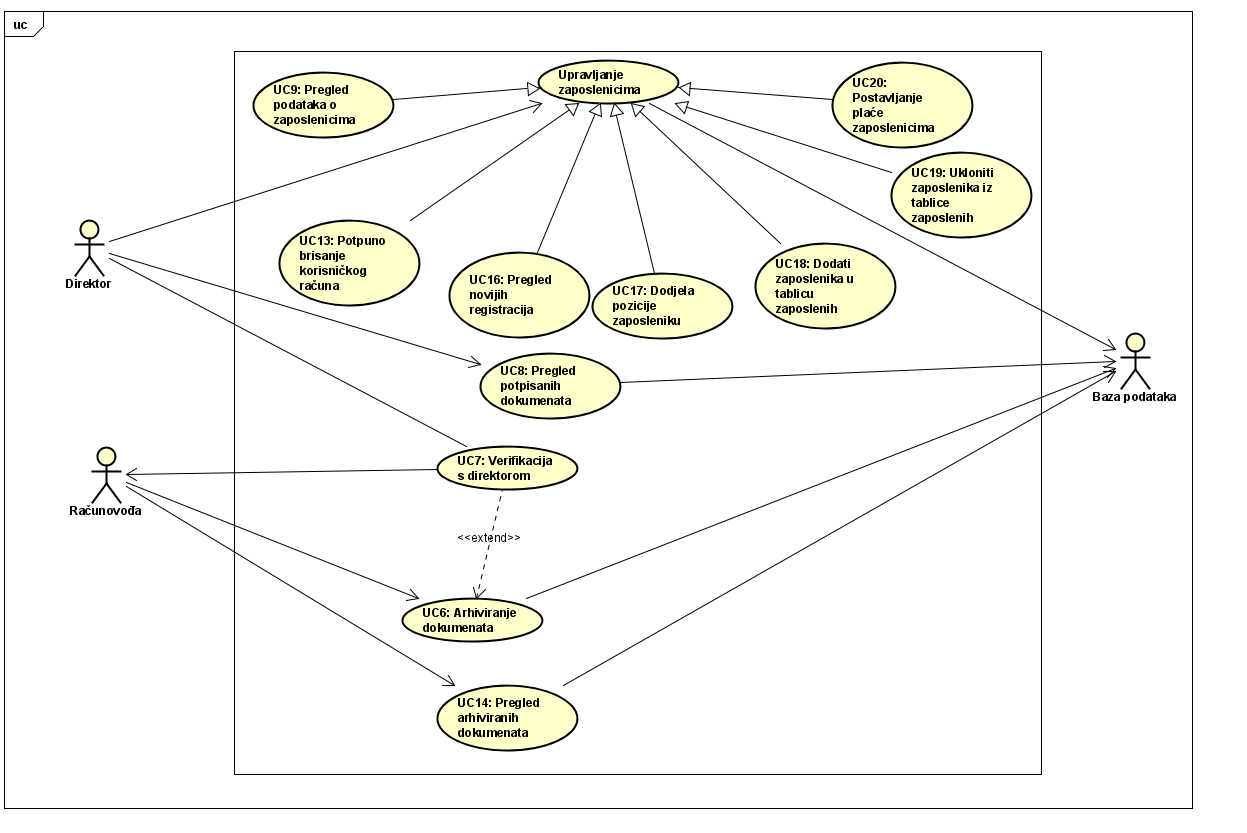
\includegraphics[scale=0.58]{slike/Direktor.png} %veličina slike u odnosu na originalnu datoteku i pozicija slike
					\centering
					\caption{Dijagram obrasca uporabe, funkcionalnost direktora i računovođe}
					\label{DUC1}
				\end{figure}
			
			
				\begin{figure}[H]
				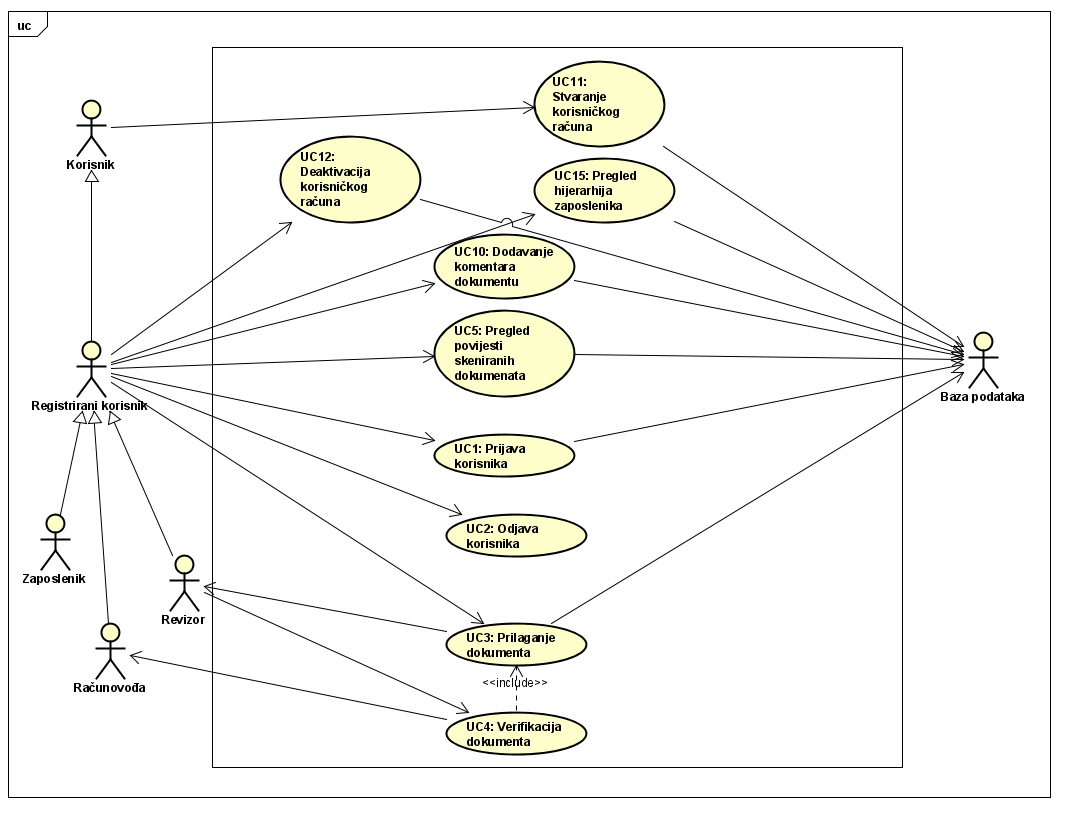
\includegraphics[scale=0.65]{slike/Korisnik.png} %veličina slike u odnosu na originalnu datoteku i pozicija slike
				\centering
				\caption{Dijagram obrasca uporabe, funcionalnost registriranih korisnika}
				\label{DUC2}
			\end{figure}				
					
			\newpage	
			\subsection{Sekvencijski dijagrami}
				
				
				Zaposlenik unosi svoje podatke kako bi se mogao prijaviti i ući u aplikaciju. Poslužitelj iz baze podataka dohvaća sve zaposlenike unutar tvrtke te traži postoji li zaposlenik s upisanim podacima. Ukoliko zaposlenik postoji u bazi podataka, zaposlenik se uspješno prijavio, a ukoliko ne postoji, poslužitelj ga šalje na stranicu registracije.
				\begin{figure}[H]
					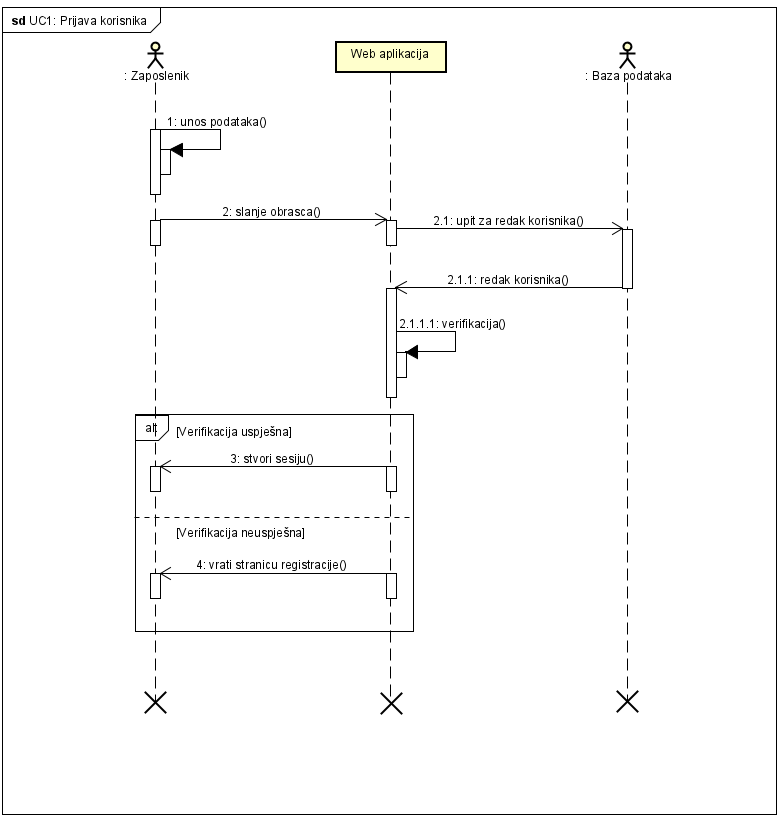
\includegraphics[scale=0.7]{slike/UC1 - Prijava korisnika.png} %veličina slike u odnosu na originalnu datoteku i pozicija slike
					\centering
					\caption{UC1 - Prijava korisnika}
					\label{uc1}
				\end{figure}
			
			\pagebreak
			Zaposlenik priloži (engl. uploada) sliku. Ima mogućnost priložiti do 50 slika. Ukoliko priloži više od 50 slika, ponavlja postupak sve dok ne priloži dozvoljeni broj. Nakon što uspješno priloži slike, slike se šalju poslužitelju koji radi OCR te zaposleniku vraća skenirani dokument. Zaposlenik ima mogućnost pogledati sve skenirane dokumente te mora označiti koji skenirirani dokumenti su ispravni te ih šalje na poslužitelj koji ih prosljeđuje revizoru na daljnju obradu.
			\begin{figure}[H]
				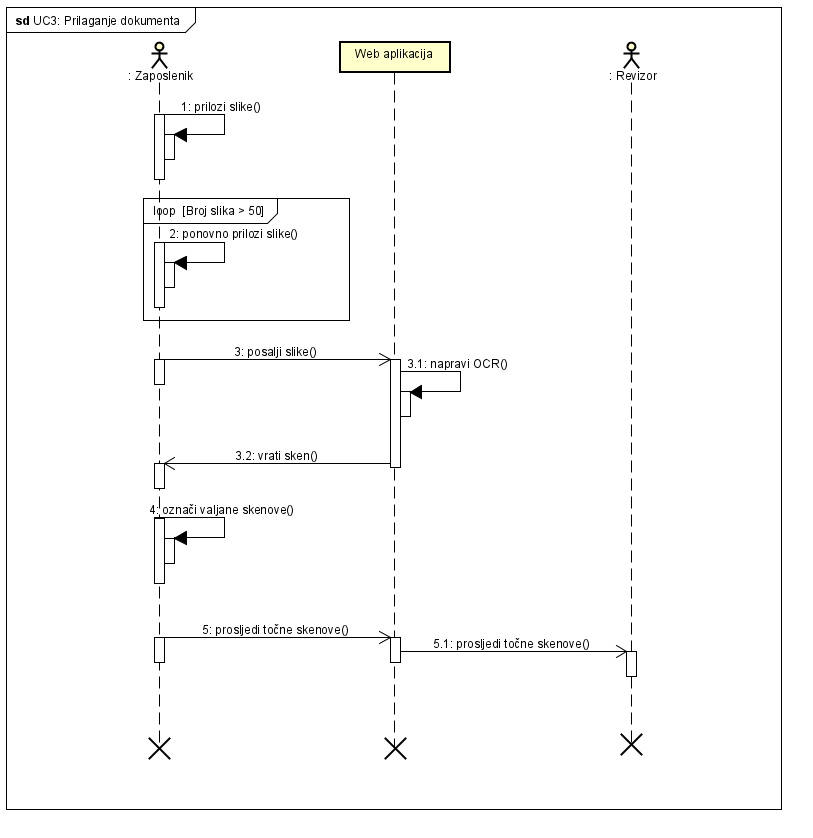
\includegraphics[scale=0.8]{slike/UC3 - Prilaganje dokumenta.png} %veličina slike u odnosu na originalnu datoteku i pozicija slike
				\centering
				\caption{UC3 - Prilaganje dokumenta}
				\label{uc3}
			\end{figure}
		\pagebreak
		Zaposlenik šalje upit poslužitelju za povijest skeniranih dokumenata. Poslužitelj upit prosljeđuje bazi podataka. Baza podataka iz tablice uzima zatražene dokumente te ih šalje poslužitelju koji ih proslijedi zaposleniku.
		\begin{figure}[H]
			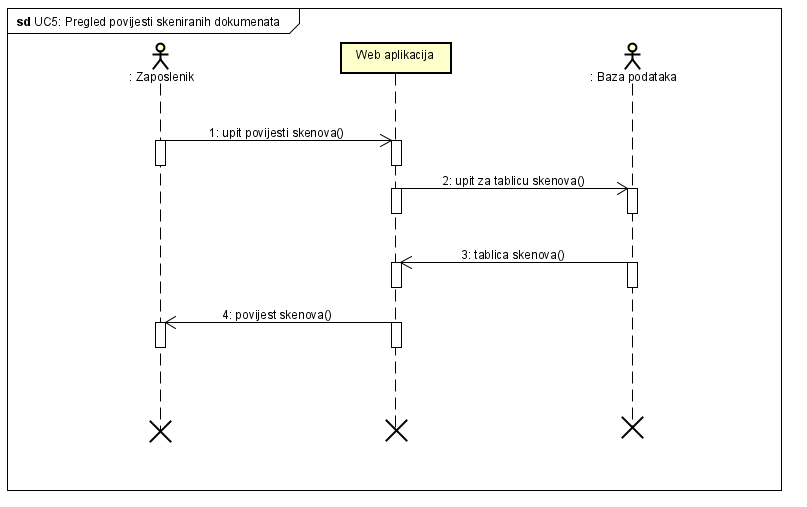
\includegraphics[scale=0.8]{slike/UC5 - Pregled povijesti skeniranih dokumenata.png} %veličina slike u odnosu na originalnu datoteku i pozicija slike
			\centering
			\caption{UC5 Pregled - povijesti skeniranih dokumenata}
			\label{uc5}
		\end{figure}
	
		\pagebreak
		Zaposlenik unosi svoje podatke. Podaci se šalju poslužitelju koji pita bazu postoji li ovaj korisnik. Ako korisnik postoji, poslužitelj korisniku javlja da je registracija pogrešna, a ako korisnik ne postoji, web poslužitelj šalje upit bazi je li zaposlenik upisao dobar jedinstveni kod. Ukoliko je kod neispravan, poslužitelj korisniku javlja da je registracija pogrešna, a ako je kod ispravan podaci se zapisuju u bazu podataka te se korisnik prosljeđuje na stranicu za prijavu.
		\begin{figure}[H]
			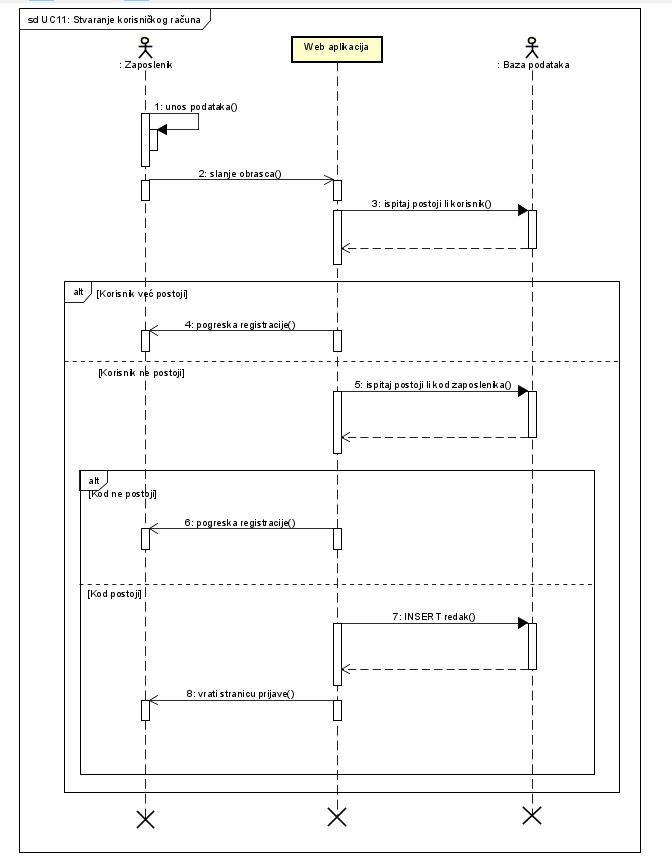
\includegraphics[scale=0.8]{slike/UC11 - Stvaranje korisnickog racuna.png} %veličina slike u odnosu na originalnu datoteku i pozicija slike
			\centering
			\caption{UC11 -  Registracija računa}
			\label{uc5}
		\end{figure}
	
		\section{Ostali zahtjevi}
			\begin{packed_item}
				 \item {Sustav treba omogućiti rad više korisnika u isto vrijeme}
				 \item {Korisničko sučelje za prijavu i registraciju moraju podržavati hrvatsku abecedu}
				 \item {Pristup sustavu mora biti omogućen iz javne mreže pomoću HTTPS (heroku deployment)}
				 \item {Ukoliko se korisnik krivo služi aplikacijom, aplikacija mora i dalje biti funkcionalna}
				 \item {Pristup bazi podataka ne smije trajati dulje od 5 sekundi}
				 \item {Sustav treba biti implementiran kao web aplikacija koristeci objektno-orijentirane jezike}
				 \item {OCR treba biti funkcionalan}
			\end{packed_item}
				
			 
			 
			 
			 
	